\documentclass[]{article}

%encoding
%--------------------------------------
\usepackage[T1]{fontenc}
\usepackage[utf8]{inputenc}
%--------------------------------------

%Portuguese-specific commands
%--------------------------------------
\usepackage[portuguese]{babel}
%--------------------------------------

%Hyphenation rules
%--------------------------------------
\usepackage{hyphenat}
\hyphenation{mate-mática recu-perar}
%--------------------------------------

% graphics package
\usepackage{graphicx}

% links to chapters
\usepackage{hyperref}

% fix references
\usepackage{notoccite}

% graphics configuration
\graphicspath{{./images/}}

\addto\captionsportuguese{
	\renewcommand{\contentsname}%
	{Índice}%
}

\begin{document}
	
\pagenumbering{roman}

\thispagestyle{empty}
	
{\centering
	
	\begin{figure}[t!]
		
\includegraphics[scale=0.5]{isel_logo}	
		\centering
	\end{figure}
	
	
	\centerline{\LARGE{INSTITUTO SUPERIOR DE ENGENHARIA DE LISBOA}}
	\bigskip
	\bigskip
	
	{ \huge \bfseries Rede Social de Voluntariado}
	\bigskip\bigskip
	
	\textbf{
		Projeto e Seminário\\
		Semestre de Verão 2019/2020\\
		Licenciatura em Engenharia Informática e de Computadores
	}
	\bigskip
	\bigskip
	
	\large \textbf{Autores:}
	\bigskip
	
	\begin{minipage}{0.4\textwidth}
		\begin{flushleft} 
			Guilherme Allen\\
			Nº 43571\\
		\end{flushleft}
	\end{minipage}
	~	
	\begin{minipage}{0.4\textwidth}
		\begin{flushright} 
			Leonardo Martins\\ 
			Nº 43591\\
		\end{flushright}
	\end{minipage}
	\bigskip
	\bigskip
	
	\large \textbf{Orientador:} Nuno Leite
	
}	

\newpage~\newpage

\section{Resumo}
(todo)

\newpage~\newpage

\section*{Abstract}
% Parágrafo intro
Nowadays, volunteering is an activity that has been gaining more prominence.
Being a volunteer promotes not only the enrichment of society but also solidarity and the value of social environments. The participation in these activities allows the volunteer to develop skills such as leadership and teamwork, which are valuable in a professional environment. \par \smallskip
% Parágrafo problemática
The divulgation and enrolment in these actions is usually done through social networks, which aren't developed with this intent in mind, and in websites, which leads to a decentralization of information. \par \smallskip
% Parágrafo descrição do projeto
Our project looks to solve these issues through the development of a social network focused on volunteering, where volunteers and organizations coexist, giving focus to the divulgation and enrolment in these actions while maintaining the typical aspects of a social network (interaction between users). The project is composed of a REST API (Javascript) and two client applications: a mobile app (Android), for the volunteers, and a web app (React), for the organizations. \par \smallskip
% Palavras chave
\textbf{Keywords}: volunteering, volunteering activities, web API, mobile app, web app.

\newpage~\newpage 

\tableofcontents
\newpage

\listoffigures
\newpage

\section{Lista de acrónimos}

\noindent \textbf{REST} Representational State Transfer \newline \smallskip

\noindent \textbf{API} Application Program Interface \newline \smallskip 

\noindent \textbf{HTTP} HyperText Transfer Protocol \newline \smallskip

\noindent \textbf{HTTPS} HyperText Transfer Protocol Secure \newline \smallskip

\noindent \textbf{NPM} Node Package Manager \newline \smallskip

\noindent \textbf{JSON} JavaScript Object Notation \newline \smallskip

\noindent \textbf{MEAN} MongoDB Express.js Angular.js Node.js \newline \smallskip 

\noindent \textbf{MERN} MongoDB Express.js React.js Node.js \newline \smallskip

\noindent \textbf{HTML} HyperText Markup Language \newline \smallskip

\noindent \textbf{CSS} Cascading Style Sheets \newline \smallskip

\noindent \textbf{SO} Sistema Operativo \newline \smallskip

\noindent \textbf{JVM} Java Virtual Machine \newline \smallskip

\newpage~\newpage~\pagenumbering{arabic}~\section{Introdução} 
Nos dias de hoje, o voluntariado é cada vez mais praticado na nossa sociedade. Segundo um estudo realizado pelo INE - Instituto Nacional de Estatística, em 2019, cerca de 6,4\% da população portuguesa realiza trabalho voluntário, uma percentagem que cresceu ligeiramente face aos resultados obtidos em 2012 (5,9\%)~\cite{INE2019}.
\par \medskip

Segundo o Diário da República, o trabalho voluntário, ou voluntariado, é definido da seguinte forma: \par \medskip

\textit{
	``O conjunto de ações de interesse social e comunitário realizadas de forma desinteressada por pessoas, no âmbito de projetos, programas e outras formas de intervenção ao serviço dos indivíduos, das famílias e da comunidade desenvolvidos sem fins lucrativos por entidades públicas ou privadas.''
}~\cite{Republica1998}

\par\medskip

Cabe assim ao voluntário (pessoa que realiza o voluntariado) e entidades o papel fulcral na sociedade de tentar enriquecer a mesma sem qualquer contrapartida. \par \medskip

Para os voluntários, a participação em ações de voluntariado permite a obtenção de competências multi-disciplinares que são valorizadas no mundo profissional, e como tal, cada vez mais empresas dão valor a candidatos que participam nestas ações. \par \medskip

Atualmente, a candidatura ao voluntariado é efetuada através de múltiplas plataformas, como redes sociais e \textit{websites}, algo que descentraliza estes serviços porque cada organização usa o seu próprio modelo (Figura 1).

\begin{figure}[h]
	\centering
	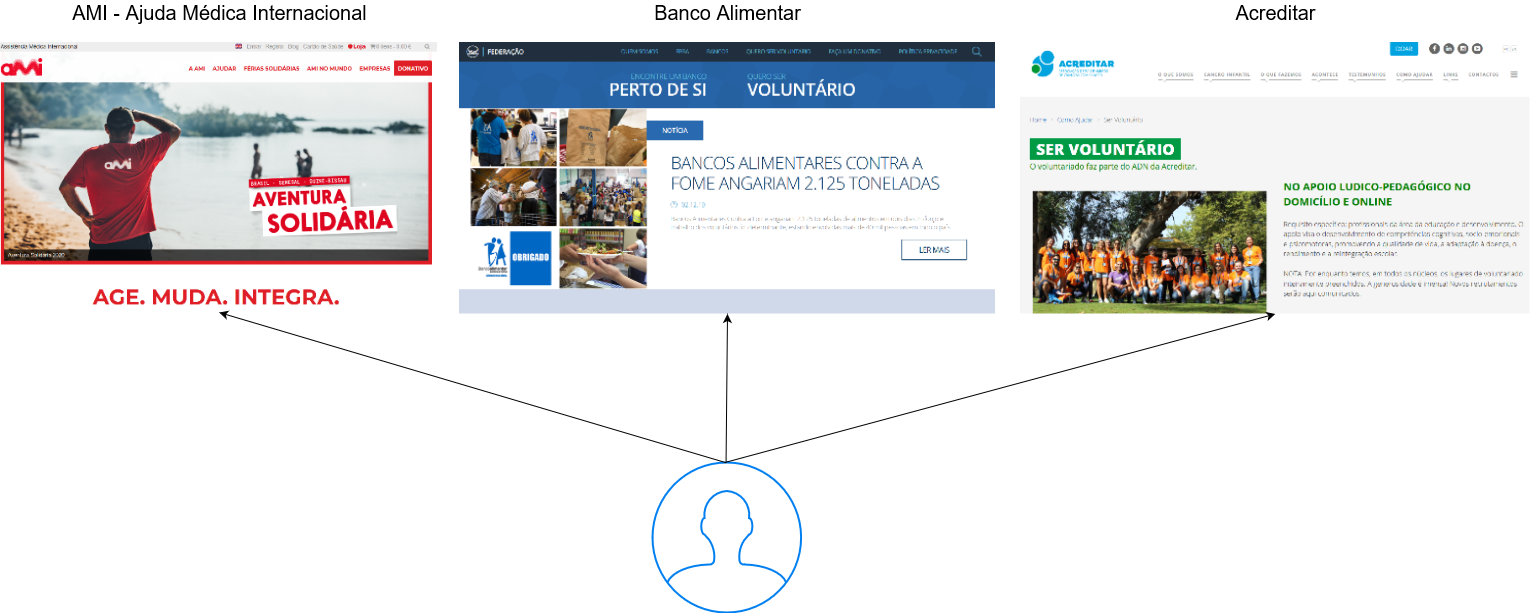
\includegraphics[scale=0.225]{services-decentralized}
	\caption{Modelo descentralizado de divulgação de voluntariado}	
\end{figure}

\newpage

O presente projeto tem como objetivo desenvolver uma rede social com foco no voluntariado. A plataforma proposta irá disponibilizar às entidades organizadoras a possibilidade de divulgar e organizar estas ações, e aos voluntários, serviços que facilitam aos mesmos manterem-se informados e participarem nas ações do seu interesse (Figura 2).

\bigskip \bigskip \bigskip

\begin{figure}[h]
	\centering
	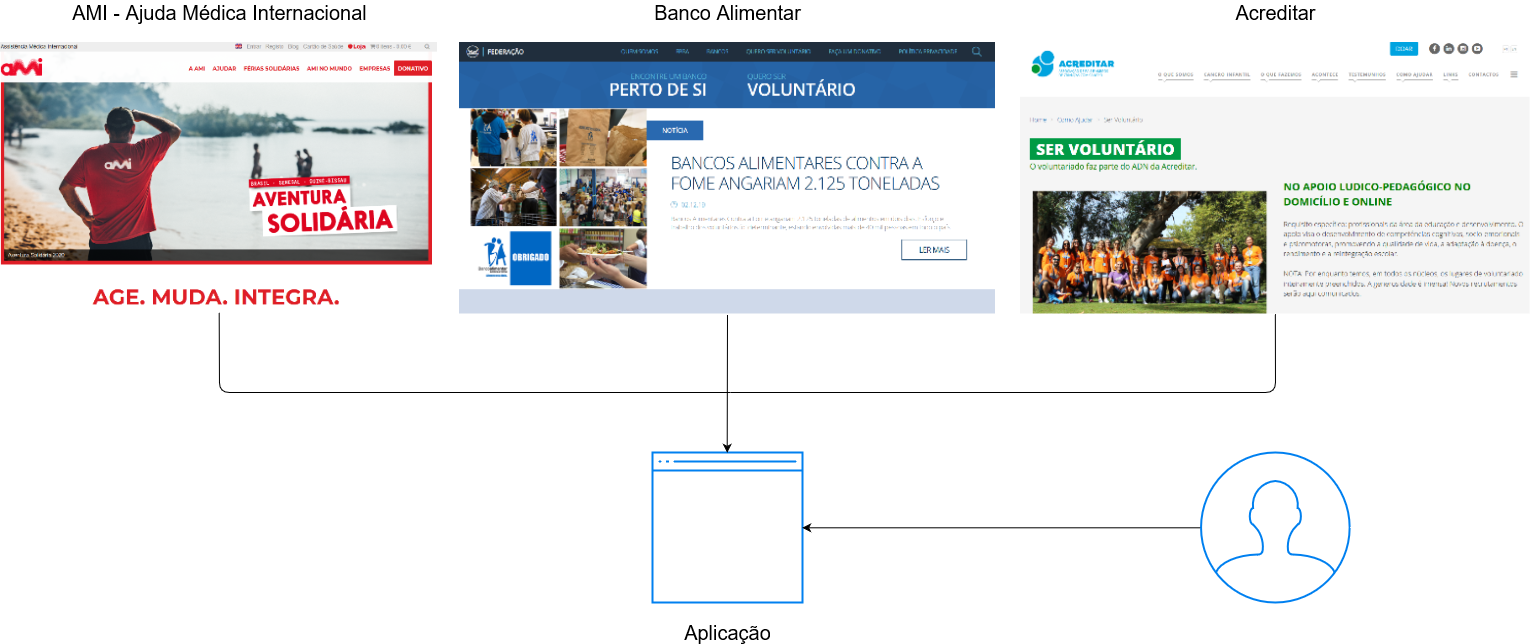
\includegraphics[scale=0.225]{services-centralized}
	\caption{Conceito do projeto}
\end{figure}

\subsection{Organização do relatório}

O restante documento encontra-se organizado em seis capítulos, descritos de seguida e pela respetiva ordem.
\begin{itemize}
	\item Formulação do problema, onde são definidos os objetivos gerais da plataforma e apresentadas outras plataformas similares. São definidos os requisitos funcionais do projeto e é escolhida a sua arquitetura;
	\item Modelo de arquitetura, capítulo responsável por discutir a arquitetura geral da plataforma e apresentar os seus módulos principais e as tecnologias utilizadas no desenvolvimento da mesma;
	\item Web API, onde é descrito o funcionamento da API usada pelas aplicações \textit{web} e móvel desenvolvidas;
	\item Mobile App, onde se aborda a implementação da aplicação cliente orientada ao voluntário;
	\item Web App, onde se apresentam detalhes relativos ao funcionamento da aplicação cliente orientada à organização;
	\item Conclusão, onde são apresentadas as conclusões tiradas após o desenvolvimento do projeto.
\end{itemize}


























\newpage

\section{Formulação do problema}

No presente capítulo, são introduzidos os elementos base que definem o sistema a desenvolver. Na secção 2.1, o problema estudado no projeto é introduzido em maior detalhe. A secção 2.2 apresenta os trabalhos relacionados com o presente projeto. Na secção 2.3 é realizada uma análise das vantagens e desvantagens das propostas existentes. Finalmente, a secção 2.4 descreve os requisitos funcionais do sistema. \par \medskip

\subsection{Problema Estudado}
A interação voluntário-organização é tipicamente feita através de dois tipos de plataformas: redes sociais (de conexões sociais) e \textit{websites} de organizações. \medskip

As redes sociais orientadas a conexões de pessoas, como por exemplo Facebook, Twitter, ou Google+, por não serem, por desenho, vocacionadas para ações de voluntariado, apresentam algumas limitações de utilização, como fraca filtragem de informação e impossibilidade de integração de múltiplas plataformas de voluntariado na mesma rede social. \medskip

Por norma, cada organização tem o seu próprio \textit{website}, algo que complica o
processo de navegação do voluntário, caso este esteja interessado em colaborar com múltiplas associações de voluntariado. \medskip

\subsubsection{Objetivos Gerais}

O projeto tem como objetivo desenvolver uma plataforma onde é disponibilizada informação relativa a ações de voluntariado, desde eventos existentes a perfis de organizações. A plataforma a desenvolver deve também auxiliar o processo de candidatura/inscrição nas ações a levar a cabo e promover a interação entre utilizadores. \medskip

A seguir descrevem-se duas plataformas que possuem objetivos semelhantes aos do presente projeto. \medskip

\subsection{Estado da Arte}

A Bolsa de Voluntariado~\cite{bolsa_voluntariado} é um projeto lançado em 2006 pela associação ENTRAJUDA com o objetivo de facilitar a procura de trabalho voluntário. \medskip

Este objetivo é concretizado através duma plataforma \textit{web} que serve de ponto de encontro entre a procura e oferta de oportunidades de voluntariado. A plataforma permite consultar ações que irão decorrer, oferecendo ainda a possibilidade aos utilizadores de as filtrarem consoante os seus interesses e visa também facilitar o processo de candidatura às mesmas. \medskip

A plataforma \textit{Online Volunteering}~\cite{online_volunteering}, desenvolvida pela UN (\textit{United Nations}) e lançada em 2000, é uma plataforma que, através do voluntariado \textit{online}, pretende reunir voluntários de múltiplas origens de maneira a auxiliarem na resolução de desafios tecnológicos das mais variadas áreas. \medskip

Esta aplicação permite a filtragem das oportunidades consoante a área de interesse e também auxilia o processo de candidatura às mesmas. 

\subsection{Análise}

Apesar destas plataformas disponibilizarem informação relativa a oportunidades de realizar trabalho voluntário e das mesmas auxiliarem a inscrição nestas ações, estas não promovem a interação entre utilizadores, que é fulcral para o crescimento de uma comunidade solidária e que leva ao aumento do número de participantes em ações de voluntariado. \medskip

Outra abordagem possível seria o desenvolvimento de uma ferramenta que aplicasse técnicas de \textit{web scraping}. Contudo, o desenvolvimento de uma ferramenta desta natureza depende da existência de fontes de informação externas e também não cumpre com a necessidade de haver interação entre utilizadores. \medskip

Uma rede social com foco em ações de voluntariado cumpre todos os objetivos descritos. Contudo, é necessário haver a migração de utilizadores para esta plataforma, algo que não é possível garantir. \medskip

Dadas as soluções apresentadas e suas vantagens/desvantagens, foi tomada a decisão de desenvolver uma rede social de voluntariado.

\subsection{Requisitos Funcionais}
O sistema a desenvolver tem os seguintes requisitos funcionais:

\begin{itemize}
	\item permitir a voluntários registarem-se, criarem um perfil e interagir com a plataforma (através da criação de \textit{posts} e sinalização de interesse em eventos);
	\item possibilitar às organizações solicitarem o registo na plataforma e também permitir às mesmas realizarem \textit{posts} e criarem eventos;
	\item mostrar às organizações os voluntários interessados nos seus eventos e disponibilizar um contacto dos mesmos (por exemplo, e-mail);
	\item garantir aos utilizadores da plataforma o acesso a interações como o seguimento de utilizadores, gostarem de \textit{posts}, entre outros.
\end{itemize}

Levando em consideração os requisitos funcionais enumerados, foi tomada a decisão de elaborar o projeto em três componentes: 
\begin{enumerate}
	\item uma \textbf{Web API}, responsável por implementar as funcionalidades necessárias para as aplicações cliente terem o comportamento pretendido. Este módulo foi desenvolvido face à necessidade de expôr os dados de forma comum a todas as aplicações cliente.
	\item Uma \textbf{aplicação móvel} orientada aos voluntários, onde os mesmos podem interagir com a plataforma. Foi tomada a decisão de desenvolver uma aplicação móvel para permitir que os voluntários possam, de maneira simples e rápida, consultar a plataforma e interagir com a mesma.
	\item Uma \textbf{aplicação \textit{web}} desenvolvida para as organizações interagirem com a plataforma, sendo que esta opção foi tomada para que múltiplos utilizadores possam gerir mais facilmente o perfil de uma organização.
\end{enumerate}
\newpage~\newpage

\section{Modelo de Arquitetura} 
O modelo do nosso projeto(demonstrado na figura 4) é constituído por três módulos principais: uma REST API, e duas aplicações cliente: uma orientada à plataforma \textit{mobile} Android e outra desenvolvida para ser usada num \textit{browser}. \par \medskip

Tendo em conta os módulos constituintes do projeto, o desenvolvimento do mesmo seguirá o standard MEAN \textit{stack} (MongoDB, Express.js, Angular, Node.js), alternando a tecnologia utilizada para desenvolver o \textit{front-end} para React em vez de Angular (também conhecido pelo MERN \textit{stack}). Foi escolhido este \textit{standard} pelas seguintes razões:
\begin{itemize}
	\item familiaridade dos autores com algumas destas tecnologias (como Express.js e Node.js);
	\item \textit{standard} utilizado no desenvolvimento de múltiplas aplicações, o que leva a uma grande quantidade de recursos;
	\item todas estas tecnologias têm em comum características que as tornam apelativas de usar conjuntamente, como por exemplo o fact da utilização de JSON ser transversal entre todas;
	\item todas as ferramentas associadas a este modelo de desenvolvimento são \textit{open-source}.
\end{itemize}

\begin{figure}[h]
	\centering
	
\includegraphics[scale=.25]{mern}
	\caption{Tecnologias do \textit{standard} MERN}
\end{figure}

Relativamente à API, esta estabelecerá endpoints onde será possível executar pedidos HTTPS de maneira a suportar autenticação e operações na infraestrutura (criação de perfil, “seguimento” de organização, inscrição em ação de voluntariado, etc.), constituindo o \textit{back-end} do projeto.
\par \medskip

Relativamente ao \textit{front-end}, serão desenvolvidas 2 aplicações cliente: 
\begin{itemize}
	\item um cliente \textit{mobile}, para a plataforma Android, usado pelos voluntários. Nesta interface será possível efetuar por parte do utilizador as operações de uso da plataforma usuais: criação de um perfil, visionamento de um \textit{feed} de \textit{posts} efetuados pelas organizações seguidas, entre outras;
	\item um cliente \textit{browser}. Esta aplicação é direcionada às organizações e terá a finalidade de permitir às mesmas realizar \textit{posts}, criar e gerir ações de voluntariado, etc.;
\end{itemize}

\begin{figure}[h]
	\centering
	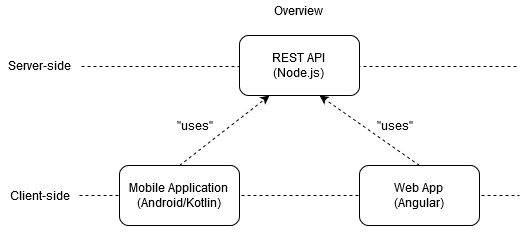
\includegraphics[scale=.8]{architecture}
	\caption{Modelo de arquitetura}
\end{figure}


\subsection{REST API}
A REST API, também definida como primeira fase do projeto, constituirá o \textit{server-side} do mesmo. É pretendido que este módulo seja completamente independente dos outros, tendo como responsabilidade trabalhar como fonte de dados para os outros componentes (client-side). \par \medskip 

A tecnologia utilizada para desenvolver este componente será Node.js em conjunto com vários package do NPM (node package manager), como o Express e o Passport. Esta escolha foi justificada por múltiplas razões:
\begin{itemize}
	\item domínio dos autores na linguagem Javascript e em vários módulos do NPM;
	\item popularidade da ferramenta, algo que simplifica o processo de desenvolvimento do componente devido à grande quantidade de recursos sobre a mesma;
	\item existência de suporte neste meio de execução de ferramentas para auxiliar o acesso à base de dados escolhida.
\end{itemize}
\par \medskip

O servidor irá ser também responsável por hospedar a base de dados, que irá funcionar no motor MongoDB. A escolha deste serviço foi efetuada devido à fácil integração do mesmo com Node.js e devido ao facto deste ter um modelo de dados baseado em documentos JSON, algo que simplifica a inserção e pesquisa sobre os mesmos.
\par \medskip

\subsection{Aplicação \textit{Mobile}}
A aplicação \textit{mobile} será desenvolvida para a plataforma Android em Kotlin. A mesma irá seguir os princípios definidos pelo Android Jetpack, que disponibiliza ferramentas e bibliotecas cujas auxiliam o desenvolvimento da aplicação. As razões que levaram a esta decisão foram:
\begin{itemize}
	\item familiaridade dos autores com esta linguagem de programação e ferramentas(Android Jetpack);
	\item a nível de quota de mercado dos sistemas operativos de dispositivos móveis, o Android é o mais prevalente;
	\item atualmente, o Kotlin é a linguagem oficial para desenvolvimento de aplicações móveis para Android.
\end{itemize}

\subsection{Aplicação \textit{Web}}
A aplicação \textit{web} será desenvolvida em React. Esta tecnologia foi escolhida devido a:

\begin{itemize}
	\item familiaridade dos autores com esta ferramenta;
	\item quota de mercado (relativamente às frameworks de Javascript utilizadas para o desenvolvimento de aplicações \textit{web}) significativa, sendo atualmente a tecnologia mais usada;
	\item integração com as outras ferramentas do projeto.
\end{itemize}

\subsection{Tecnologias e ferramentas}
As seguintes tecnologias irão ser utilizadas durante o desenvolvimento do projeto:
\begin{itemize}
	\item \textbf{Javascript}: Principal linguagem para programação client-side em browsers; Esta é tipicamente utilizada em conjunto com ferramentas como o HTML e CSS para implementar a funcionalidade de uma página web;
	\item \textbf{Node.js}: Interpretador e ambiente de execução para Javascript normalmente utilizado para executar código sem ser num cliente browser;
	\item \textbf{NPM}: package manager do Javascript/Node.js;
	\item \textbf{Express}: web framework para Node.js. Auxilia o processo de routing e definição de endpoints, encapsulando aspetos do HTTP, para tornar mais fácil o desenvolvimento de \textit{Web} APIs;
	\item \textbf{Passport}: Middleware de autenticação usado em conjunto com o Express para simplificar o processo de autenticação e gestão de sessões de utilizadores;
	\item \textbf{MongoDB}: Base de dados noSQL baseada em documentos JSON. Tipicamente integrada com Javascript devido à natureza dos seus documentos;
	\item \textbf{Android}: Sistema operativo open source para dispositivos móveis desenvolvido pela Google. Atualmente, cerca de 75\% dos dispositivos móveis usam este SO;
	\item \textbf{Kotlin}: Linguagem de programação desenvolvida pela JetBrains que compila para a JVM. Atualmente, o Kotlin é a linguagem oficial do Android;
	\item \textbf{Android Jetpack}: Conjunto de ferramentas e bibliotecas as quais auxiliam a implementação e desenvolvimento de software para o sistema operativo móvel Android;
	\item \textbf{React}: Biblioteca \textit{open-source} de Javascript usada para desenvolver a UI de aplicações.
\end{itemize}
\newpage

\section{API}

Neste capítulo, é dado ênfase ao desenvolvimento da API. Como tal, é realizada uma introdução, onde são definidos os requisitos da mesma e são, de maneira reduzida, referidas as tecnologias utilizadas no desenvolvimento desta. De seguida, é apresentada a conceptualização da plataforma e as operações que esta suporta, passando posteriormente para a definição da sua arquitetura e seus sub-módulos. O capítulo é concluído com a realização de uma referência relativamente à base de dados e ao \textit{deployment} da plataforma.

\medskip \par

A \textit{web} API é responsável por estabelecer um serviço RESTful~\cite{Fielding2000} com o qual é possível comunicar sobre HTTPS e que implementa as funcionalidades da plataforma. Esta constitui o \textit{back-end} do projeto e como tal, funciona como fonte de dados para as aplicações cliente.

\medskip \par

Este módulo necessita de cumprir um conjunto de requisitos:

\begin{itemize}
	\item implementar as funcionalidades pretendidas da plataforma, como obtenção de listas de voluntários, registo por parte de utilizadores e outras operações;
	\item interagir com a base de dados;
	\item comunicar sobre HTTPS e suportar autenticação por parte dos clientes.
\end{itemize}

\medskip \par

Tendo em conta o \textit{stack} tecnológico selecionado para desenvolver este projeto, a API foi  desenvolvida em Typescript (sendo que o código é compilado para Javascript) e a mesma é instanciada usando Node.js~\cite{Wilson2018}.

\subsection{Conceptualização}

Tendo em consideração que está a ser desenvolvida uma rede social de voluntariado, foi necessário definir as entidades que estariam disponíveis na plataforma. 

\par \medskip

Relativamente aos utilizadores da plataforma, foram constituídos dois tipos: \textbf{voluntários} e \textbf{organizações}. É necessário haver esta distinção dado que na organização de uma ação de voluntariado estes são dois dos sujeitos participantes mais importantes: aqueles que a organizam (organizações) e aqueles que auxiliam a mesma voluntariamente (voluntários).

\par \medskip

Sendo o propósito da plataforma divulgar este tipo de ações - é necessário definir mais uma entidade: \textbf{eventos}. Estes representam eventos de voluntariado (organizados por organizações registadas na plataforma) que já ocorreram ou que irão ocorrer. É importante também definir que voluntários podem colocar-se como \textit{interessados} num evento - sendo que a partir do momento que estes o façam, é disponibilizado à organização dona do evento o seu contacto.

\par \medskip

Dada a natureza da plataforma é necessário permitir que os utilizadores da plataforma (voluntários e organizações) possam ter uma identidade social de maneira a distinguirem-se dos outros. Sendo assim, foi definido que os utilizadores podem editar o seu perfil (com descrições, contatos e imagens) e realizar \textit{\textbf{posts}}, sendo possível a outros interagir com estes aspetos (na forma de \textit{gostar de posts} e \textit{seguir outro utilizador}).
 
\subsection{Operações}

Levando em consideração o conceito da plataforma definido anteriormente, inicializou-se então a constituição de funcionalidades da API. Definiram-se operações (invocadas através de \textit{endpoints}) que permitem a clientes da plataforma interagir com a mesma, na forma de:

\begin{itemize}
	\item consultar voluntários, organizações, \textit{posts} e eventos;
	\item possibilitar que utilizadores possam criar e editar o seu perfil;
	\item criar \textit{posts} e eventos;
	\item seguir outros utilizadores, gostar de \textit{posts} e ainda marcar o interesse num evento.
\end{itemize}

A referência a todas estas operações encontra-se na \href{https://github.com/leomartins1999/PS1920-G46/wiki}{\textit{wiki}} do projeto.

\subsection{Arquitetura}

A \textit{Web} API, representada na Figura 5, é composta por três módulos: \textbf{controladores}, \textbf{serviços} e \textbf{repositórios} e ainda uma classe principal, responsável por inicializar o servidor e efetuar configurações relacionadas com autenticação e definição de \textit{endpoints}~\cite{Lauret2019,Block2014}.

\begin{figure}[h]
	\centering
	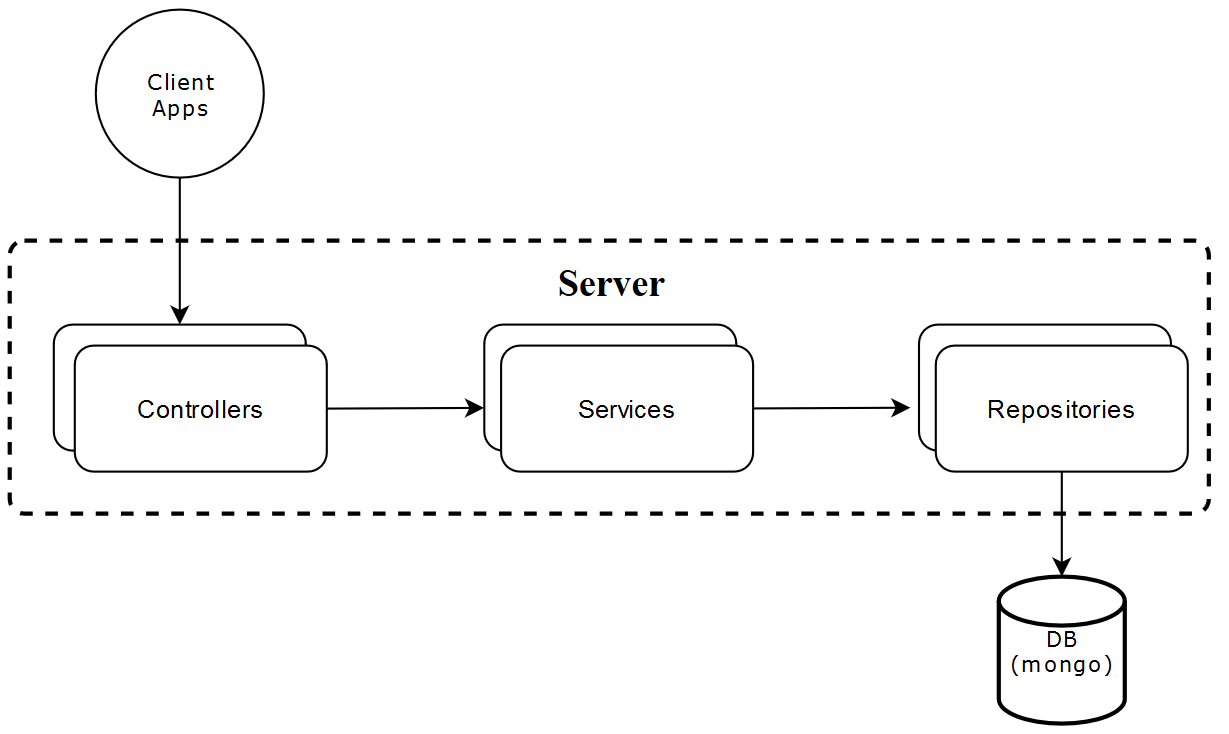
\includegraphics[scale=.30]{api_architeture}
	\caption{Diagrama de arquitetura da API.}
\end{figure}

Resumidamente, os \textbf{controladores} têm como responsabilidade a definição de \textit{endpoints} e a realização de chamadas aos serviços, sendo que estes últimos (\textbf{serviços}) tratam a implementação da lógica da aplicação e realização de chamadas aos repositórios. Estes (\textbf{repositórios}) são responsáveis por interagir com a base de dados.

\subsubsection{Controladores}

Tal como já referido, estes definem os \textit{endpoints} existentes na API e invocam o serviço correspondente. No início da execução da aplicação, é instanciado um controlador para cada entidade existente (voluntários, organizações, \textit{posts} e eventos), sendo que nessa instanciação são definidos \textit{endpoints} utilizando o mecanismo de encaminhamento (\textit{routing}) do Express.

\medskip \par

Os controladores tratam também de recolher os parâmetros provenientes nos pedidos HTTPS (contidos no caminho, na \textit{query string}, no corpo do pedido e na sessão do utilizador) e passar os mesmos às funções do serviço, sendo que independentemente do sucesso ou não destas, estes lidam também com a realização das respostas HTTPS.

\subsubsection{Serviços}

Para cada controlador, existe associado a este um serviço. Neste, são definidas as funções que o controlador invoca de maneira a executar a operação pretendida pelo cliente da API.

\medskip \par

Todos os serviços têm uma relação hierárquica de extensão com um serviço base, onde se encontram definidos estaticamente os repositórios de acesso à base de dados. 

\medskip \par

Os serviços, fazendo uso dos repositórios, interagem com a base de dados para implementar a lógica das operações, sendo que o resultado destas é devolvido assincronamente ao controlador.

\subsubsection{Repositórios}

Os repositórios têm como função interagir com a base de dados e devolver o resultado das operações efetuadas assincronamente ao serviço, de maneira a este cumprir a operação solicitada.

\medskip \par

Cada objeto repositório contém uma referência para uma instância de repositório base. Este repositório base é definido genericamente e contém a implementação de operações CRUD sobre a base de dados.

\subsubsection{Autenticação}

De maneira a garantir que os clientes da aplicação possam ter uma experiência personalizada, esta API suporta autenticação através do uso de Passport.js, configurado de maneira a fazer uso de \textit{web cookies}. A partir do momento que um utilizador tem sucesso no processo de autenticação na plataforma, todos os seus pedidos contêm informação relativamente à sessão do mesmo.

\medskip \par

Certas operações na API estão protegidas de maneira a que utilizadores não autenticados não as possam efetuar (como por exemplo a realização de um \textit{post} ou a alteração de um perfil). De maneira a que um utilizador possa aceder a estas, é necessário que este tenha realizado autenticação previamente (e por sua vez, tenha realizado registo na plataforma anteriormente) e que o cliente \textit{web} utilizado por este suporte a utilização de \textit{cookies}.

\subsection{Base de dados}

Tal como introduzido anteriormente, foi tomada a decisão de utilizar MongoDB. MongoDB é um motor de base de dados noSQL~\cite{mongoDB2020}, isto é, apresenta um modelo não relacional através da utilização de coleções e documentos.

\medskip \par

Esta escolha implica que todos os documentos numa coleção não necessitam de ter a mesma estrutura, algo que traz alguma flexibilidade e agilidade no processo de desenvolvimento sobre esta plataforma. Outra característica interessante é que os documentos seguem o formato JSON, simplificando a integração destes dados com a aplicação (devido ao uso de Javascript).

\medskip \par

O motor foi selecionado não só para hospedar os dados associados às entidades mas também para albergar o conteúdo das imagens fornecidas pelos utilizadores.

\subsection{Implantação da API}

Tendo em consideração o meio em que o projeto foi desenvolvido, foi tomada a decisão de hospedar a base de dados na máquina onde está implantada (\textit{deployed}) a API (hospedada no serviço Compute Engine da Google Cloud Platform). Contudo, seria mais interessante do ponto de vista de escalabilidade se a mesma fosse hospedada remotamente (através de uma solução \textit{cloud} como o Amazon Web Services ou a Google Cloud Platform) porque possibilitaria a instanciação de múltiplas aplicações API, e consequentemente, a realização de balanceamento de carga.

\medskip \par

A máquina virtual foi configurada com os recursos necessários (como o Node.js) e, numa primeira fase, a aplicação foi instanciada para testes. De maneira a atribuir um nome de domínio ao endereço IP da máquina, foi utilizado o serviço Duck DNS e de seguida, utilizando o CertBot, foi emitido um certificado SSL de maneira a garantir que fosse possível a instanciação da aplicação num modo em que as comunicações fossem realizadas sobre o protocolo HTTPS. A utilização deste protocolo torna a realização de comunicações entre cliente e servidor mais segura devido à encriptação da informação trocada entre ambos. Em plataformas nas quais ocorre a troca de dados sensíveis (como palavras-passe) entre cliente e servidor é essencial a utilização deste protocolo~\cite{Cloudflare2020}.







\newpage

\section{\textit{Mobile App}}
O desenvolvimento deste componente ainda não foi inicializado. No entanto, está previsto que à data da entrega da versão \textit{beta}, a implementação dos requisitos funcionais deste módulo esteja completa.
\newpage~\newpage

\section{\textit{Web App}}

Neste capítulo é abordado o desenvolvimento da aplicação \textit{web}. É realizada uma introdução, apresentando os objetivos e funcionalidades da mesma. São mostrados detalhes relativos à utilização da aplicação e, de seguida, apresenta-se o modelo de arquitetura utilizado no desenvolvimento da mesma. Por fim, refere-se como aceder à aplicação e define-se o seu processo de \textit{deployment}.

\par \smallskip

A aplicação \textit{web} é responsável por estabelecer uma interface sobre a qual as organizações podem interagir com a plataforma, disponibilizando às mesmas ferramentas que possibilitam a realização de operações como por exemplo a criação de \textit{posts} ou a realização de pesquisas sobre a plataforma.

\par \smallskip

Foram definidos alguns requisitos chave no início da conceptualização da aplicação, como por exemplo:

\begin{itemize}
	\item disponibilizar meios para consultar os \textit{posts}, eventos e outros utilizadores da plataforma e interagir com os mesmos; 
	\item permitir às organizações editarem o seu perfil;
	\item possibilitar que as mesmas possam criar e editar \textit{posts} e eventos;
	\item apresentar contactos de voluntários interessados em eventos pertencentes à organização autenticada.
\end{itemize}

Numa fase inicial do projeto, foi considerada a opção de desenvolver a aplicação \textit{web} usando a \textit{framework} Angular.js. Contudo, após nova avaliação, optou-se por utilizar a tecnologia React~\cite{Stefanov2016}. Esta alteração foi efetuada após verificar que React é a tecnologia mais usada no mercado à data da realização do projeto. 

\subsection{Utilização da web app}

Levando em consideração que este componente foi desenvolvido especificamente para organizações, a maioria das operações implicam que um utilizador organização esteja autenticado (através da interface demonstrada na Figura 9).

\begin{figure}[h]
	\centering
	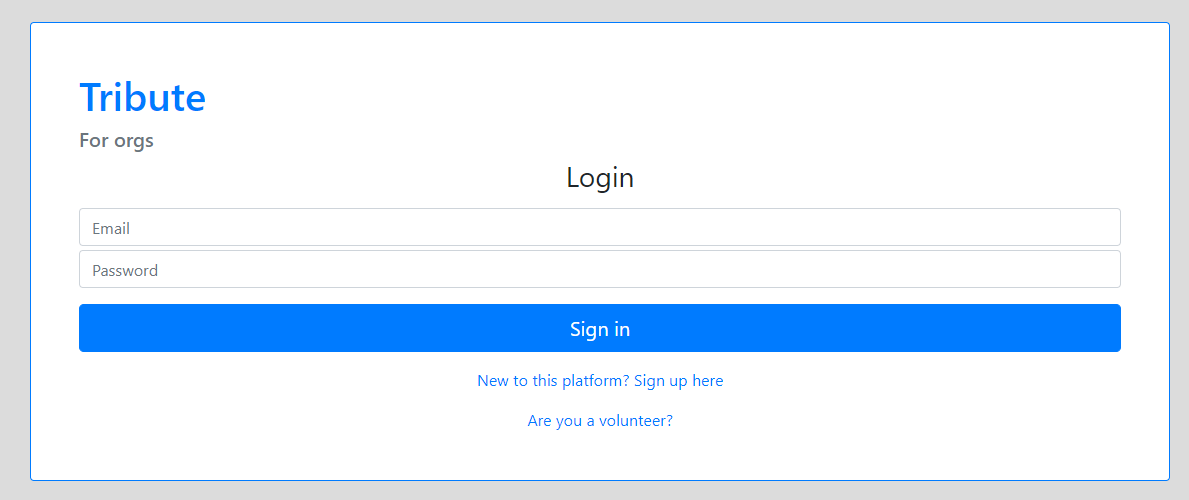
\includegraphics[scale=.31]{web_app_login_page}
	\caption{Interface de autenticação}
\end{figure}

Nesta versão da aplicação, é permitido que sejam registados utilizadores do tipo organização. Contudo, numa versão publicada da plataforma, o registo deste tipo de utilizadores seria realizado através do contacto direto dos mesmos com os gestores da aplicação de maneira a que apenas organizações fidedignas pudessem ter um perfil na plataforma.

\par \medskip

\begin{figure}[h]
	\centering
	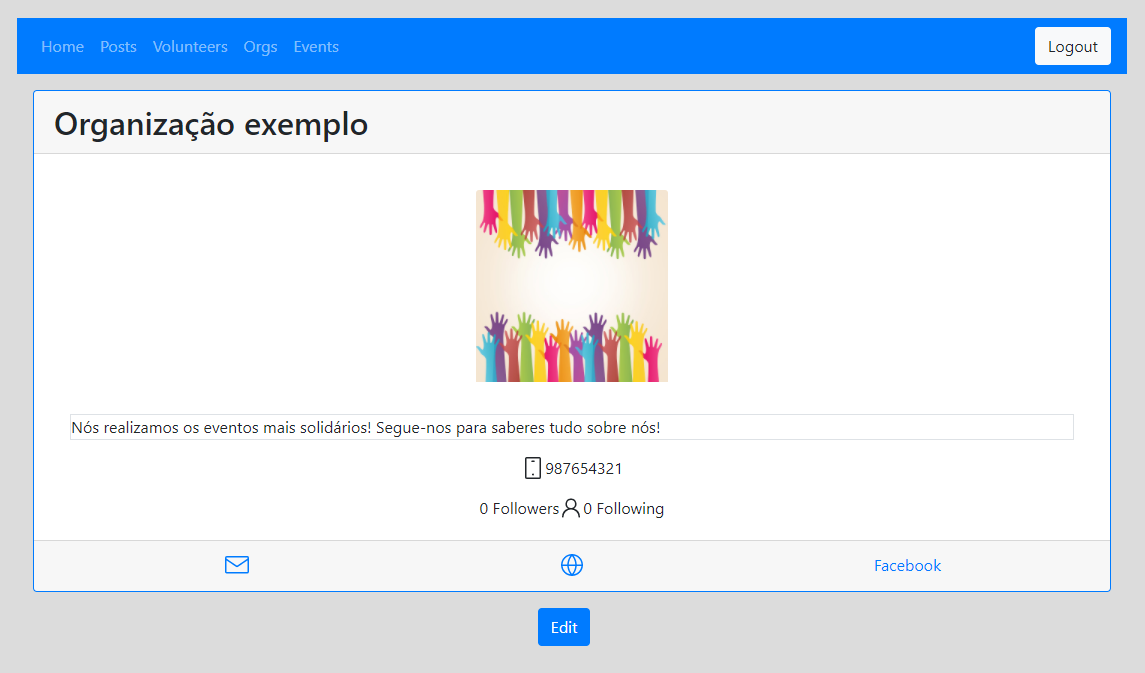
\includegraphics[scale=.39]{web_app_dashboard}
	\caption{Interface de autenticação}
\end{figure}

Após autenticação na aplicação, é disponibilizado um painel principal (consultar Figura 10) onde é possível navegar entre as várias páginas da aplicação e realizar as operações pretendidas.

\par \medskip

\subsection{Arquitetura}

A arquitetura da aplicação é composta principalmente por 2 módulos: API e Componentes e ainda a classe principal da aplicação.

\par \medskip 

Similar ao funcionamento do módulo com o mesmo nome na aplicação \textit{mobile}, API disponibiliza operações que realizam pedidos HTTPS à API. Componentes contém a implementação de todos os componentes \textit{react} apresentados ao utilizador, desde as páginas em si a componentes que são utilizados nestas. 

\par \medskip

A classe principal da aplicação é responsável não só por instanciar os serviços da API assim como definir o roteamento da aplicação \textit{web}.

\subsubsection{API}

A módulo API é composto por um conjunto de serviços que disponibilizam operações que necessitam de realizar pedidos HTTPS à API para serem realizadas (como por exemplo a solicitação de \textit{posts} ou a criação de um evento).

\par \medskip

Para cada entidade (voluntários, organizações, \textit{posts} e eventos) existe um serviço onde são definidas as operações possíveis de efetuar sobre a mesma. Todos os serviços utilizam uma classe auxiliar que contém a implementação de como efetuar pedidos HTTPS consoante o seu método (neste caso, GET, PUT, POST e DELETE). Esta classe auxiliar contém também a implementação de um requests

\subsubsection{Componentes}

Tal como já referido, o módulo Componentes é responsável por tratar a estruturação e apresentação da interface da aplicação assim como lidar com operações de \textit{input} por parte do utilizador. Como tal, este contém a definição de:

\begin{itemize}
	\item \textbf{componentes página}. Estes componentes definem os sub-componentes que constituem a página (por exemplo, na figura 11, a página dos eventos é constituída por um formulário para criar um novo evento e a lista dos eventos existentes na plataforma);
	\item \textbf{componentes específicos} por página, como por exemplo, uma lista de \textit{posts} ou um formulário para criar eventos;
	\item \textbf{componentes utilitários}, responsáveis por apresentar certos aspetos comuns da aplicação.
\end{itemize}

\begin{figure}[h]
	\centering
	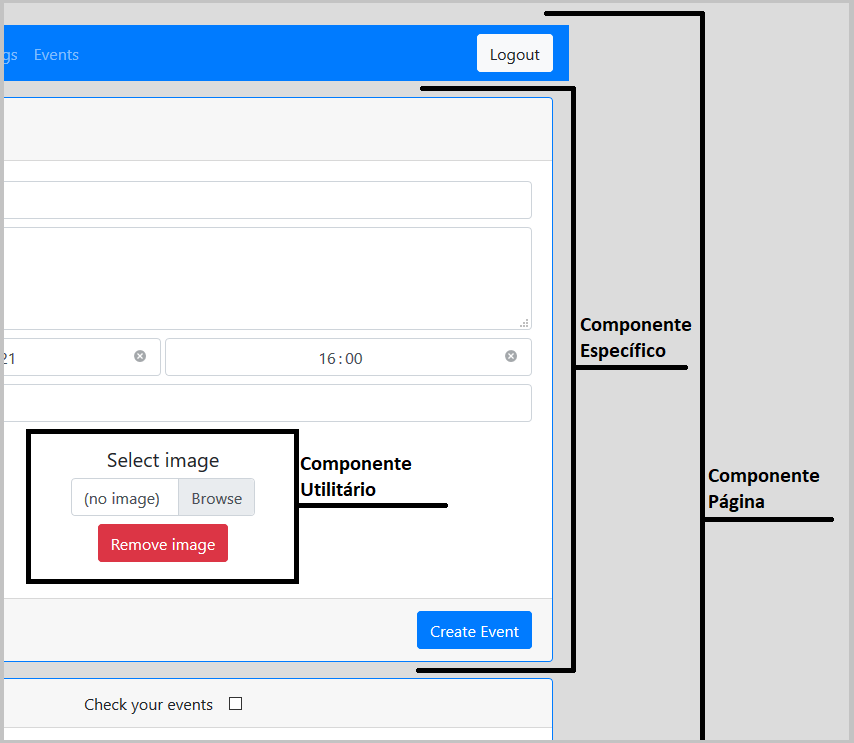
\includegraphics[scale=.43]{components_explained}
	\caption{Exemplo de tipos de componentes na página dos eventos}
\end{figure}

\bigskip

\subsubsection{Classe Principal}

A classe principal da aplicação instancia os serviços usados pelos componentes para efetuar pedidos à API e define também o roteamento da aplicação \textit{web}. No modo não autenticado, o acesso a quase todas as rotas da aplicação web é restringido. Apenas quando o cliente realiza autenticação com sucesso é permitido ao mesmo aceder às funcionalidades principais da aplicação.

\subsection{\textit{Deployment} da aplicação}

A aplicação foi \textit{deployed} utilizando uma máquina virtual do serviço \textit{Compute Engine} da \textit{Google Cloud Platform}. Foram instaladas as ferramentas necessárias para executar a aplicação nesta máquina (nomeadamente \textit{Node.js}) e a mesma encontra-se instanciada numa das portas da VM. 

\par \medskip

De maneira a lidar com pedidos CORS (Cross-Origin Resource Sharing), na máquina onde é executada a aplicação está instanciado um servidor \textit{web} Nginx. Este está configurado de maneira a redirecionar todos os pedidos que comecem com o preâmbulo /api para a máquina onde está \textit{deployed} a \textit{web} API. Todos os outros pedidos são redirecionados para a porta onde está a ser executada a aplicação \textit{web}.

\par \medskip

De maneira a associar um nome de domínio ao endereço IP da máquina onde está a ser executado o servidor \textit{web} foi utilizada a plataforma \textit{Duck DNS}, que permite reservar sem qualquer custo um número limitado de \textit{domain names}.

\par \medskip

Por fim, e utilizando as ferramentas disponibilizadas pela plataforma \textit{CertBot}, foi automaticamente emitido um certificado SSL e alterada a configuração do servidor \textit{Nginx} de maneira a que a plataforma aceitasse apenas comunicações através do protocolo HTTPS, garantindo segurança ponto-a-ponto entre máquina cliente e servidor \textit{web}.

\par \medskip

A aplicação encontra-se acessível em \url{https://tribute-app.duckdns.org/}.
















































\newpage

\section{Conclusão}
À data da entrega do relatório de progresso, podemos apontar algumas conclusões a partir daquilo que foi o desenvolvimento do componente API:

\begin{itemize}
	\item apesar dos conhecimentos relativamente à implementação de uma API já obtidos ao longo da licenciatura, tivemos alguma dificuldade naquilo que foi o desenho e definição de requisitos funcionais da API. Após uma primeira versão da mesma, voltámos a implementá-la uma segunda vez, esta com uma estrutura melhor definida e que cumpre todas as funcionalidades que um cliente da API irá necessitar;
	\item como já foi referido, apesar da mesma já ter sido consolidada uma segunda vez, podemos necessitar de adicionar alguns componentes extra aquando do desenvolvimento das aplicações cliente, sendo que estes componentes extra irão surgir quando forem necessários.
\end{itemize}
\newpage

% bibliography
\bibliographystyle{unsrturl}
\bibliography{bibrefs}

\end{document}





